\documentclass[conference]{IEEEtran}
\IEEEoverridecommandlockouts
% The preceding line is only needed to identify funding in the first footnote. If that is unneeded, please comment it out.
\usepackage{cite}
\usepackage{amsmath,amssymb,amsfonts}
\usepackage{algorithmic}
\usepackage{graphicx}
\usepackage{textcomp}
\usepackage[table]{xcolor}
\usepackage{xcolor}
\def\BibTeX{{\rm B\kern-.05em{\sc i\kern-.025em b}\kern-.08em
    T\kern-.1667em\lower.7ex\hbox{E}\kern-.125emX}}
\begin{document}

\title{Deep Reinforcement Learning usage in games playing\
}

\author{\IEEEauthorblockN{ Andrew Zakhary}
\IEEEauthorblockA{\textit{Electronics Engineering} \\
\textit{Hochschule Hamm-Lippstadt}\\
Hamm, Germany \\
2210009}
}





\maketitle

\begin{abstract}

\end{abstract}

\begin{IEEEkeywords}
Deep learning, Reinforcement learning, artificial intelligence, video games
\end{IEEEkeywords}

\section{Introduction}
Games have been a large part of our human society and history from the beginning. Evidence was found that early humans used $Talus bones$ as rudimentary dice as early as 10,000 years B.C\cite{10.1007/978-981-10-0575-6_1       }. As human society developed so did the games they played. The first board game found was in the Levant, dating back to around 7,500 years ago \cite{simpson2007earliest} with a couple of rows of holes carved into limestone. from then on board games developed more complexity from the relative simplicity of games as $Mancala$ in the Mediterranean to $Senet$ in Egypt to $Go$ in chine, which is the  oldest board game of mental skill in the world that is still being played\cite{shotwell1994game}. Games like $Go$ and $Chess$ (previously $chatarunga$) captivated the minds of humans for centuries because they are so complex that no one human could ever master them. This is due to the vast number of possible variations in a single game. In chess for example a typical game is around 40 moves, this could lead $10^{120}$ possible positions according to Claude Shanon\cite{shannon1950xxii}.

In the last decades though, games have found their renaissance with the new technological revolution. The invention of the computer allowed games to take on a new shape. It's highly argued what could count as the first $video game$ because the exact definition of the word $game$ is contested. what could be said with certainty though is that video games started around the 1950s in research facilities. After that video games became commercially available such as $Computer Space$ in 1971 and $Pong$ in 1971. $Pong$ Specially was importan for the fact that the user could play against a computer system (commonly known as $Game-AI$ afterwards). From the late 80s and early 90s video games established themselves as a mean of entertainment and art. The growing capabilities of computers allowed the creation of more complex games till our current day.

With the growing computational power available also came the need for more powerful AI systems. AI systems developments proved to be essential for developing solutions that would have been very difficult using normal computational methods. In recent history multiple methods for developing such systems as supervised learning, unsupervised learning, reinforcement learning, deep learning and transfer learning among many others. A lot of effort has been put recently in the scope of developing AI systems that can play video games by themselves. This is due to the fact that video games can be a stepping stone in generating AI systems that have ability to work alongside humans in their tasks. Similar to the real world, many video games have an environment where the player is free to do a set of actions and only at the end of a set of time would he know if he was successful or not. The AI model would then need to learn the patterns that succeed and and unlearn the patterns that don't. This is why methods as Reinforcement Learning and Deep Reinforcement Learning are ideal in many video games playing situations. In this paper the workings of a Deep Reinforcement Learning model is explained as well as showing an implementation of such a model using a $Python$ script.
\section{Basic Concepts}
\subsection{Reinforcement learning}
Unlike other approaches of creating AI models where there's a correct and wrong answers, Reinforcement learning is useful where answers are not binary but rather can lead do different levels of success. This can be exemplified by the different tasks of identifying a cat from a dog and playing a game like Snake. In the former, for each image there's a correct and incorrect solution while in the later, there's various degrees of success for each attempt. In Reinforcement Learning, the system can be split into two parts Agent and Environment. The Environment produces all the information about the state of the system. This collection of information is called $state$. The agent takes in the $state$, process it and depending on the internal model generates a corresponding output called $action$, The environment is also responsible for returning a $reward$ depending on the $action$ produced by the agent. A s
\begin{figure}
    \centering
    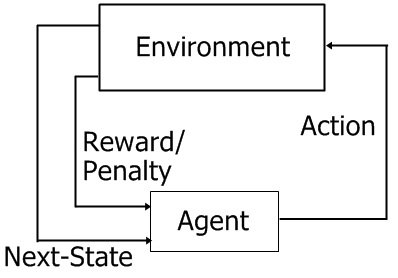
\includegraphics[width=0.5\linewidth]{Reinforcement-Learning-block-diagram.png}
    \caption{Overview of an RL model\cite{inproceedings}}
    \label{fig:RL}
\end{figure}


Agent perfroms Actions in the Environment, gets Reward and calculates the next Action
signal (S,a,r) are called experience. 
at max time the set of experiences collected is called trajectory, the period of time is called an episode.

\section{Implementation}

\subsection{Methodology}

\subsection{Example}

\section{Conclusion}
\bibliographystyle{unsrt} 
\bibliography{refs}

\end{document}
